\chapter{Функционал неавторизованного пользователя}
    \section{Общие элементы страниц}
        \subsection{Фиксированная панель слева}
            См. рис. \ref{fig:common_items_1}

            \label{sec:baseitems_fixleft_panel}
            \subsubsection{Логотип}
                См. рис. \ref{fig:common_items_2}

                \begin{enumerate}
                   \item Ссылка с логотипа на главную страницу
                \end{enumerate}
            \subsubsection{Кнопки соцсетей}
                См. рис. \ref{fig:common_items_2}

                \begin{enumerate}
                    \item Ссылка на группу вконтакте http://vk.com/citizenmoscow
                    \item Ссылка на страницу в facebook https://www.facebook.com/citizenmoscow
                    \item Ссылка на аккаунт в twitter https://twitter.com/citizenmoscow
                    \item Ссылка на страницу в instagram https://instagram.com/citizenmoscow/
                \end{enumerate}
            \subsubsection{Кнопка <<вверх>>}
                См. рис. \ref{fig:common_items_2}
                \begin{enumerate}
                    \item На главной и в разделах каталога при нажатии перематывает страницы к фильтру. 
                    \item На вторичных страницах перематывает страницу к началу(к главному меню)
                \end{enumerate}
        \subsection{Главное меню}
            См. рис. \ref{fig:common_items_1}

            \label{sec:baseitems_main_meu}
            \subsubsection{Ссылка на каталог}
                \begin{enumerate}
                    \item Адрес ссылки /catalog/
                    \item Ссылка активна на всех разделах каталога /catalog/*
                \end{enumerate}
            \subsubsection{Ссылка на правила.}
                \begin{enumerate}
                    \item Адрес ссылки /rules/
                    \item С /rules/ идет редирект на /rules/hiw/ (см. \ref{sec:rules_hiw})
                    \item Ссылка активна на всех разделах каталога /rules/*
                \end{enumerate}
            
            \subsubsection{Форма поиска}
                \begin{enumerate}
                    \item Placeholder - <<поиск>>
                    \item Отправка запроса на поиск по нажатию <<Enter>>
                    \item Переход на страницу поиска (\ref{sec:search_page}) при отправке формы
                \end{enumerate}

       \subsection{Важные ссылки}
            \label{sec:baseitems_important_links}
            См. рис. \ref{fig:common_items_2}

            \subsubsection{О проекте}
                \begin{enumerate}
                    \item Ссылка указывает на страницу <<как это работает>> (\ref{sec:rules_hiw})
                \end{enumerate}
            \subsubsection{Часто задаваемые вопросы}
                \begin{enumerate}
                    \item Ссылка указывает на страницу <<faq>> (\ref{sec:page_faq})
                \end{enumerate}
            \subsubsection{Обратная связь.}
                См. рис. \ref{fig:common_items_3}

                \begin{enumerate}
                    \item Ссылка вызывает модальное окно-\gloss{FBF} без перезагрузки страницы
                    \item \gloss{FBF} скрывается кликом на кнопку <<отмена>> или по нажатию <<Esc>>
                    \item Форма имеет два поля для заполнения <<тип обращения>> и <<сообщение>>.
                    \item Сообщение не отправляется, если не заполнено поле <<сообщение>>, выводится сообщение с просьбой заполнить это поле
                    \item Сообщение не отправляется, если не выбрано значение в поле <<тип обращения>>, выводится сообщение с просьбой заполнить это поле
                    \item Доступные типы обращений: <<другое>>.
                    \item После успешной отправки выводится сообщение об успехе и модальное окно с формой закрывается
                    \item После не успешной отправки выводится сообщение об ошибке и модальное окно с формой остается на месте
                \end{enumerate}

        \subsection{Копирайт}
            \label{sec:baseitems_footer_copiright}
            См. рис. \ref{fig:common_items_2}

            \begin{enumerate}
                \item Текст <<(C) 2016, Активный гражданин, Все права защищены. Публичная оферта>>
                \item Ссылка с <<Публичная оферта>> на <<faq>> (\ref{sec:page_faq})
            \end{enumerate}

        \begin{figure}
            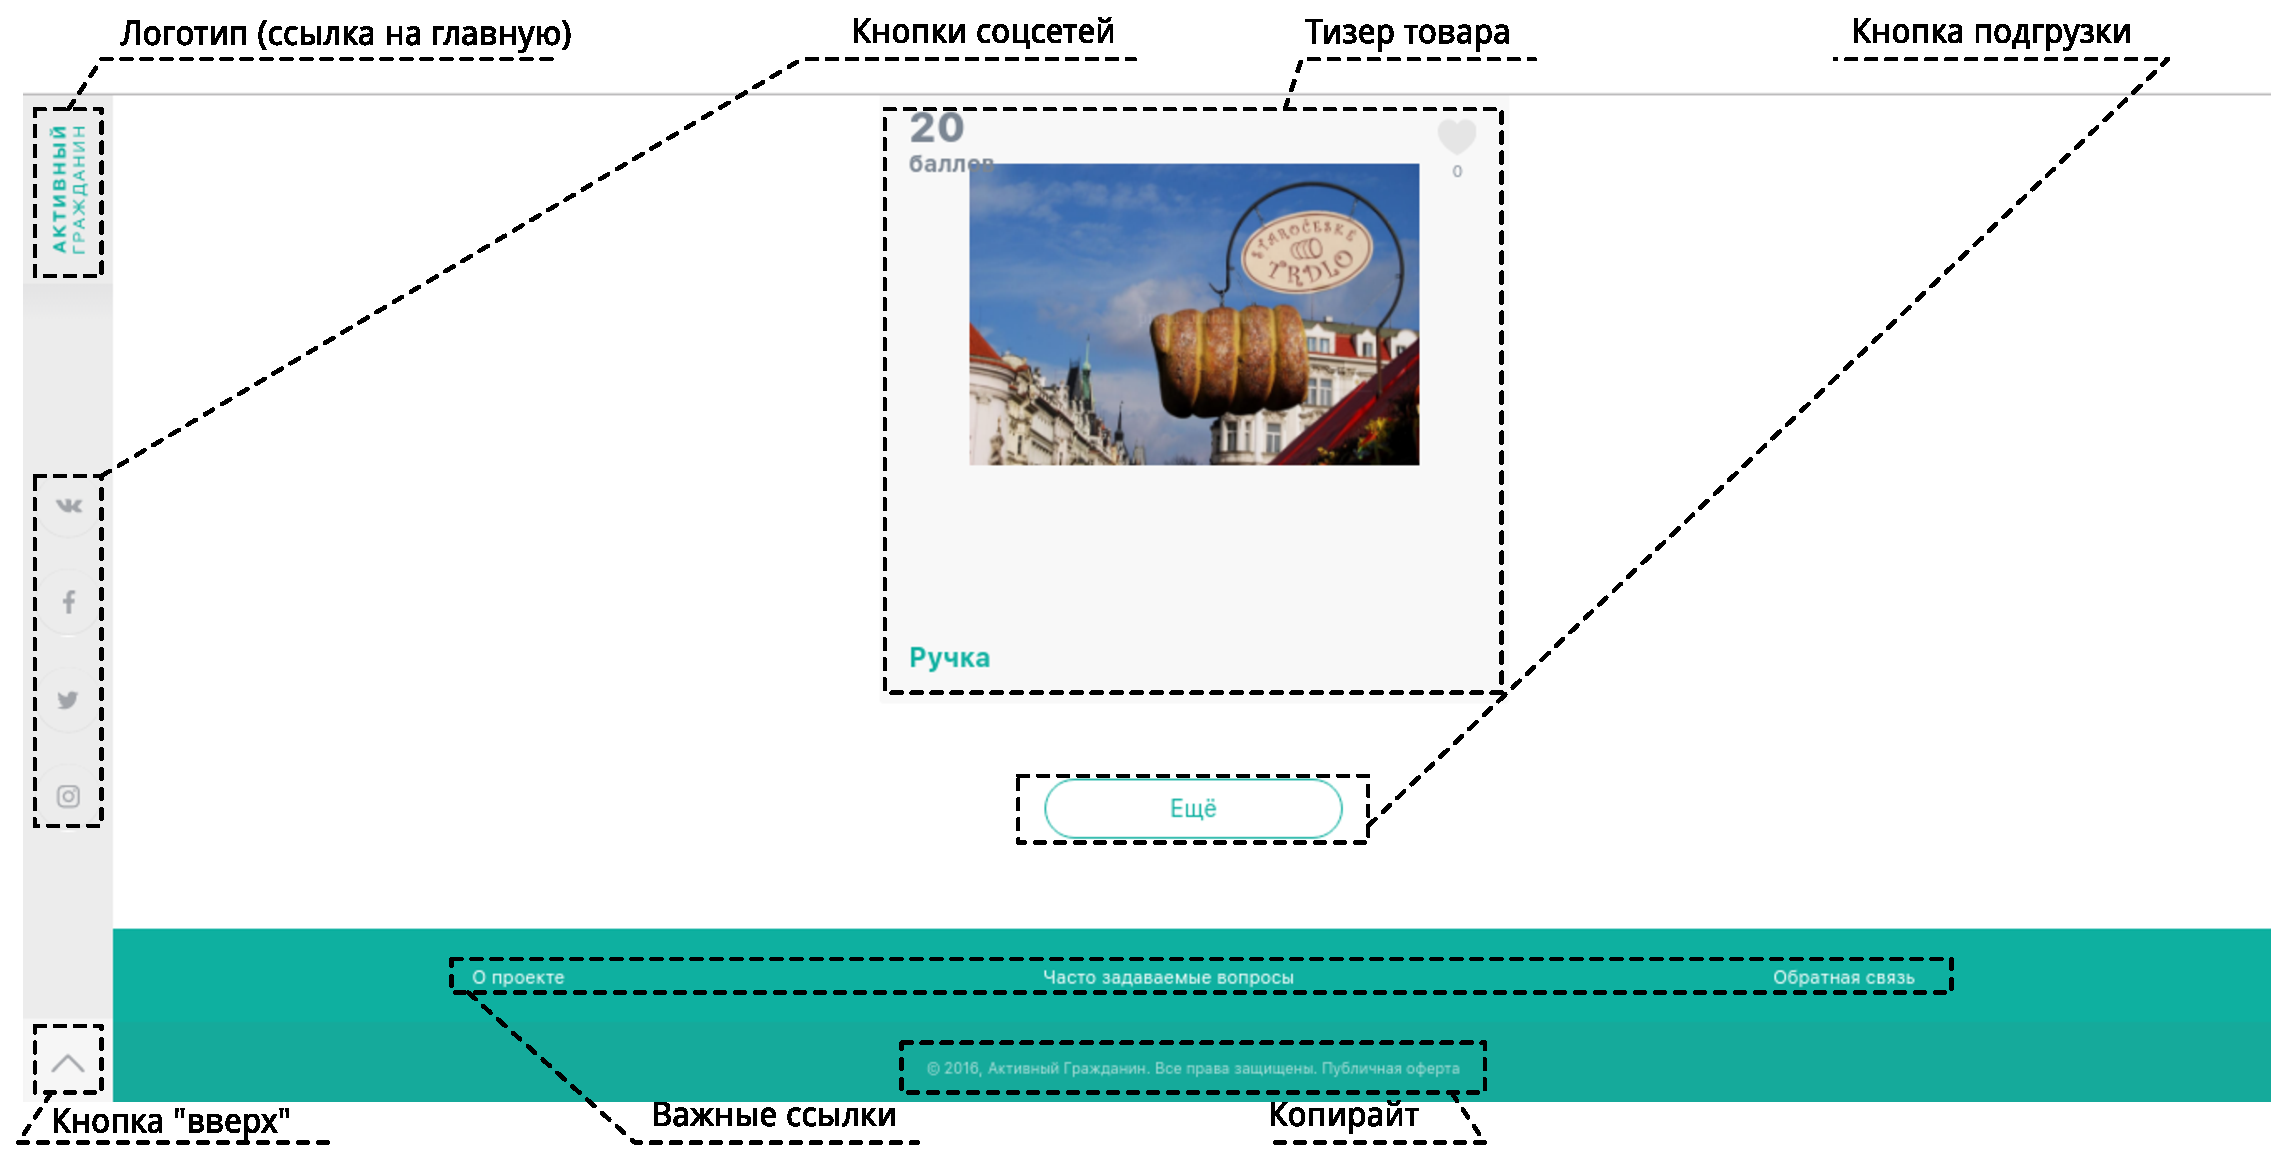
\includegraphics[width=170mm]{02_noauth_funcs/figures/03r.eps}
            \caption{Общие элементы страниц(нижняя часть страницы) и тизер товара.}
            \label{fig:common_items_2}
        \end{figure}
        \begin{figure}[h]
            \center
            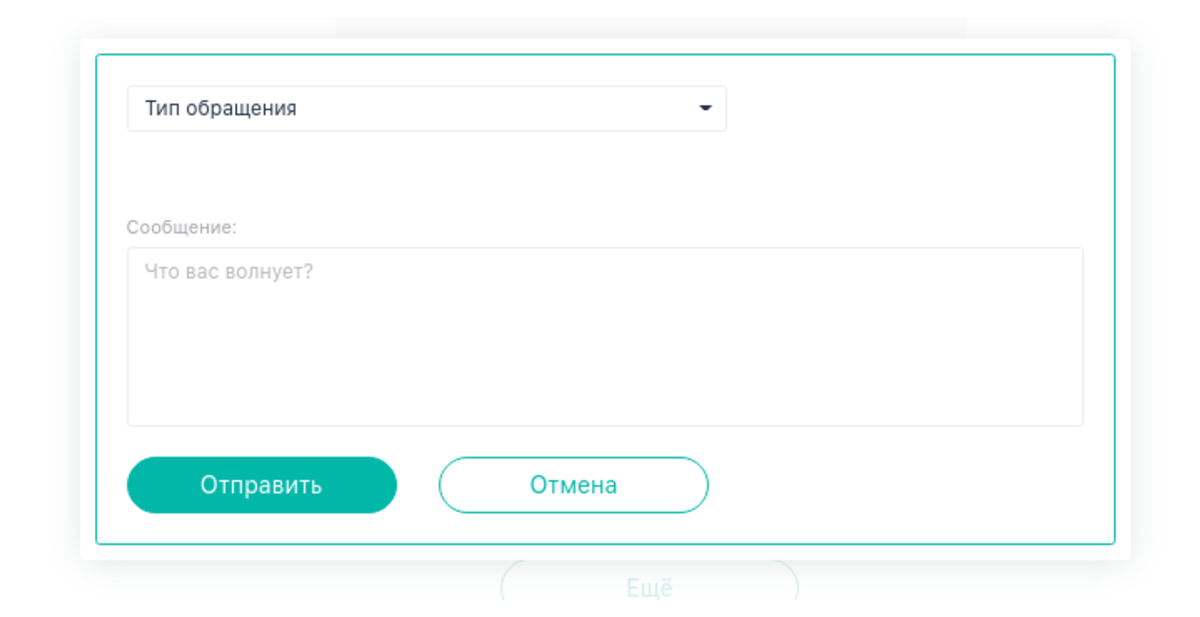
\includegraphics[width=100mm]{02_noauth_funcs/figures/04.eps}
            \caption{Форма обратной связи.}
            \label{fig:common_items_3}
        \end{figure}

        \subsection{Меню разделов магазина}
            См. рис. \ref{fig:common_items_1}

            \begin{enumerate}
                \item В меню разделов магазина входят только те разделы, которые имеют товары со свойством <<Включено>>(ACTIVE)
                \item Каждый из пунктов имеет ссылку страницу раздела каталога (2.3) вида /catalog/<траслит имени раздела>/
                \item Пункт меню активен при нахождении на соответствующей странице раздела каталога (\ref{sec:page_catalog_section})
            \end{enumerate}
        \subsection{Фильтр по цене и интересам}
            См. рис. \ref{fig:common_items_5}

            \label{sec:baseitems_interest_filter}
            \begin{enumerate}
                \item При клике по заголовку каждой из вкладок, открывается поле с выбором элементов-кнопок, имеющих
                    отношение к этой вкладке
                \item Вкладки <<хочу>> и <<интересуюсь>> соответствуют одноименным свойствам товаров, вкладка <<баллы>>
                    --- свойству цена.
                \item В каждой вкладке можно выбрать не более 3 кнопок, при попытке выбрать 4-ю выводится сообщение и 
                    выбор не происходит
                \item Отмена выбора элемента-кнопки осуществляется повторным нажатием по ней
                \item При выборе элемента кнопки происходит обновление области вывода тизеров товаров (см. \ref{sec:baseitems_goods_area}) в соответствии с 
                    выбранным набором кнопок во всех вкладках.
                \item Фильтрация элементов в области вывода тизеров товаров (см. \gloss{goods_tizer}) происходит по
                    правилу <<логическое ИЛИ>> в пределах одной вкладки и <<логическое И>> между вкладками. То есть
                    (хочу развиваться ИЛИ кататься) И (интересуюсь музыкой ИЛИ модой)
                \item если внутри одной вкладке не выбрано ни одной кнопки --- это равноценно выбору всех.
            \end{enumerate}
            \subsubsection{Вкладка <<хочу>>}
                Содержит следующие элементы для выбора: 
                \begin{enumerate}
                    \item развиваться; 
                    \item кататься; 
                    \item на мероприятие; 
                    \item развлечься; 
                    \item на природу;
                    \item экскурсию;
                    \item романтики;
                    \item что-то на память.
                \end{enumerate}
            \subsubsection{Вкладка <<интересуюсь>>}
                Содержит следующие элементы для выбора: 
                
                \begin{enumerate}
                    \item изобретениями;
                    \item животными;
                    \item фотографией;
                    \item физикой;
                    \item историей;
                    \item строительством;
                    \item музыкой;
                    \item физиологией;
                    \item культурой;
                    \item архитектурой;
                    \item космосом;
                    \item гастрономией;
                    \item природой;
                    \item спортом;
                    \item искусством;
                    \item технологиями;
                    \item модой.
                \end{enumerate}
            \subsubsection{Вкладка <<баллы>>}
                Для неавторизованного пользователя заменяется на ссылку <<войти>>, ведущую к форме авторизации на
                \gloss{AG}
                
        \subsection{Ссылки фильтра по флагам}
            См. рис. \ref{fig:common_items_5}

            \label{sec:baseitems_props_filter}
            Каждый из товаров имеет следующие свойства-флаги, отображаемые на тизере (см. \gloss{goods_tizer}) иконками:
            \begin{enumerate}
                \item хит;
                \item акция;
                \item новое.
            \end{enumerate}
            При клике по соответствующей ссылке в области вывода тизеров остаются только те товары, у которых установлен
            соответствующий флаг.

        \subsection{Ссылки сортировки списка тизеров товаров}
            См. рис. \ref{fig:common_items_5}
            \label{sec:baseitems_goods_sort}

            Порядок вывода тизеров (см. \gloss{goods_tizer}) в области вывода тизеров товаров можно установить, кликнув
            по одной из ссылок:
            \begin{enumerate}
                \item сначала дешевые;
                \item сначала дорогие;
                \item сначала популярные.
            \end{enumerate}


        \subsection{Область вывода тизеров товаров}
            См. рис. \ref{fig:common_items_5}
            \label{sec:baseitems_goods_area}

            Динамически подгружаемая область страницы, в которую выводятся тизеры товаров (см. \gloss{goods_tizer})
            согласно выбранному разделу товаров (см. \ref{sec:page_catalog_section}), установленным элементам выбора фильтра по цене и интересам (см.
            \ref{sec:baseitems_interest_filter}), фильтру по флагам (см. \ref{sec:baseitems_props_filter}) и сортируются
            согласно выбранному в п. \ref{sec:baseitems_goods_sort} порядку.

        \subsection{Кнопка подгрузки.}
            см. рис. \ref{fig:common_items_2}

            Служит для вывода новой порции тизеров товаров в область вывода.

            \label{sec:baseitems_goods_more}
        \subsection{Тизер товара}
            см. рис. \ref{fig:common_items_4}

            \subsubsection{Цена}
                Цена товара в баллах.
            \subsubsection{Иконка <<хит>>}
                Выводится, если у товара выставлен флаг <<лидер продаж>>
            \subsubsection{Иконка <<новое>>}
                Выводится, если у товара выставлен флаг <<новинка>>
            \subsubsection{Иконка <<акция>>}
                Выводится, если у товара выставлен флаг <<спецпредложение>>
            \subsubsection{Число желающих}
                Цифра показывает сколько пользователей группы 
                \glossary{auth_user} выбрали этот товар в качестве желаемого 
                кликом на сердечко. Неавторизованный пользователь может видеть
                эту цифру, но не может добавить товар в желаемое
            \subsubsection{Средняя оценка}
                Показывает среднюю оценку(от 0 до 5), которую поставили пользователи, 
                заказавшие данный товар
            \subsubsection{Раздел}
                Информационный элемент, показывающий принадлежность товара к разделю.
                Некликабелен.
            \subsubsection{Название}
                Название товара.
            \subsubsection{Изображение}
                Основное изображение. При необходимости масштабируется, чтобы 
                полностью помещаться в тизере.
            \subsubsection{Описание}
                Описание товара. При необходимости обрезается до 128 символов, 
                чтобы не вылезать за пределы тизера


        \begin{figure}[h]
            \center
            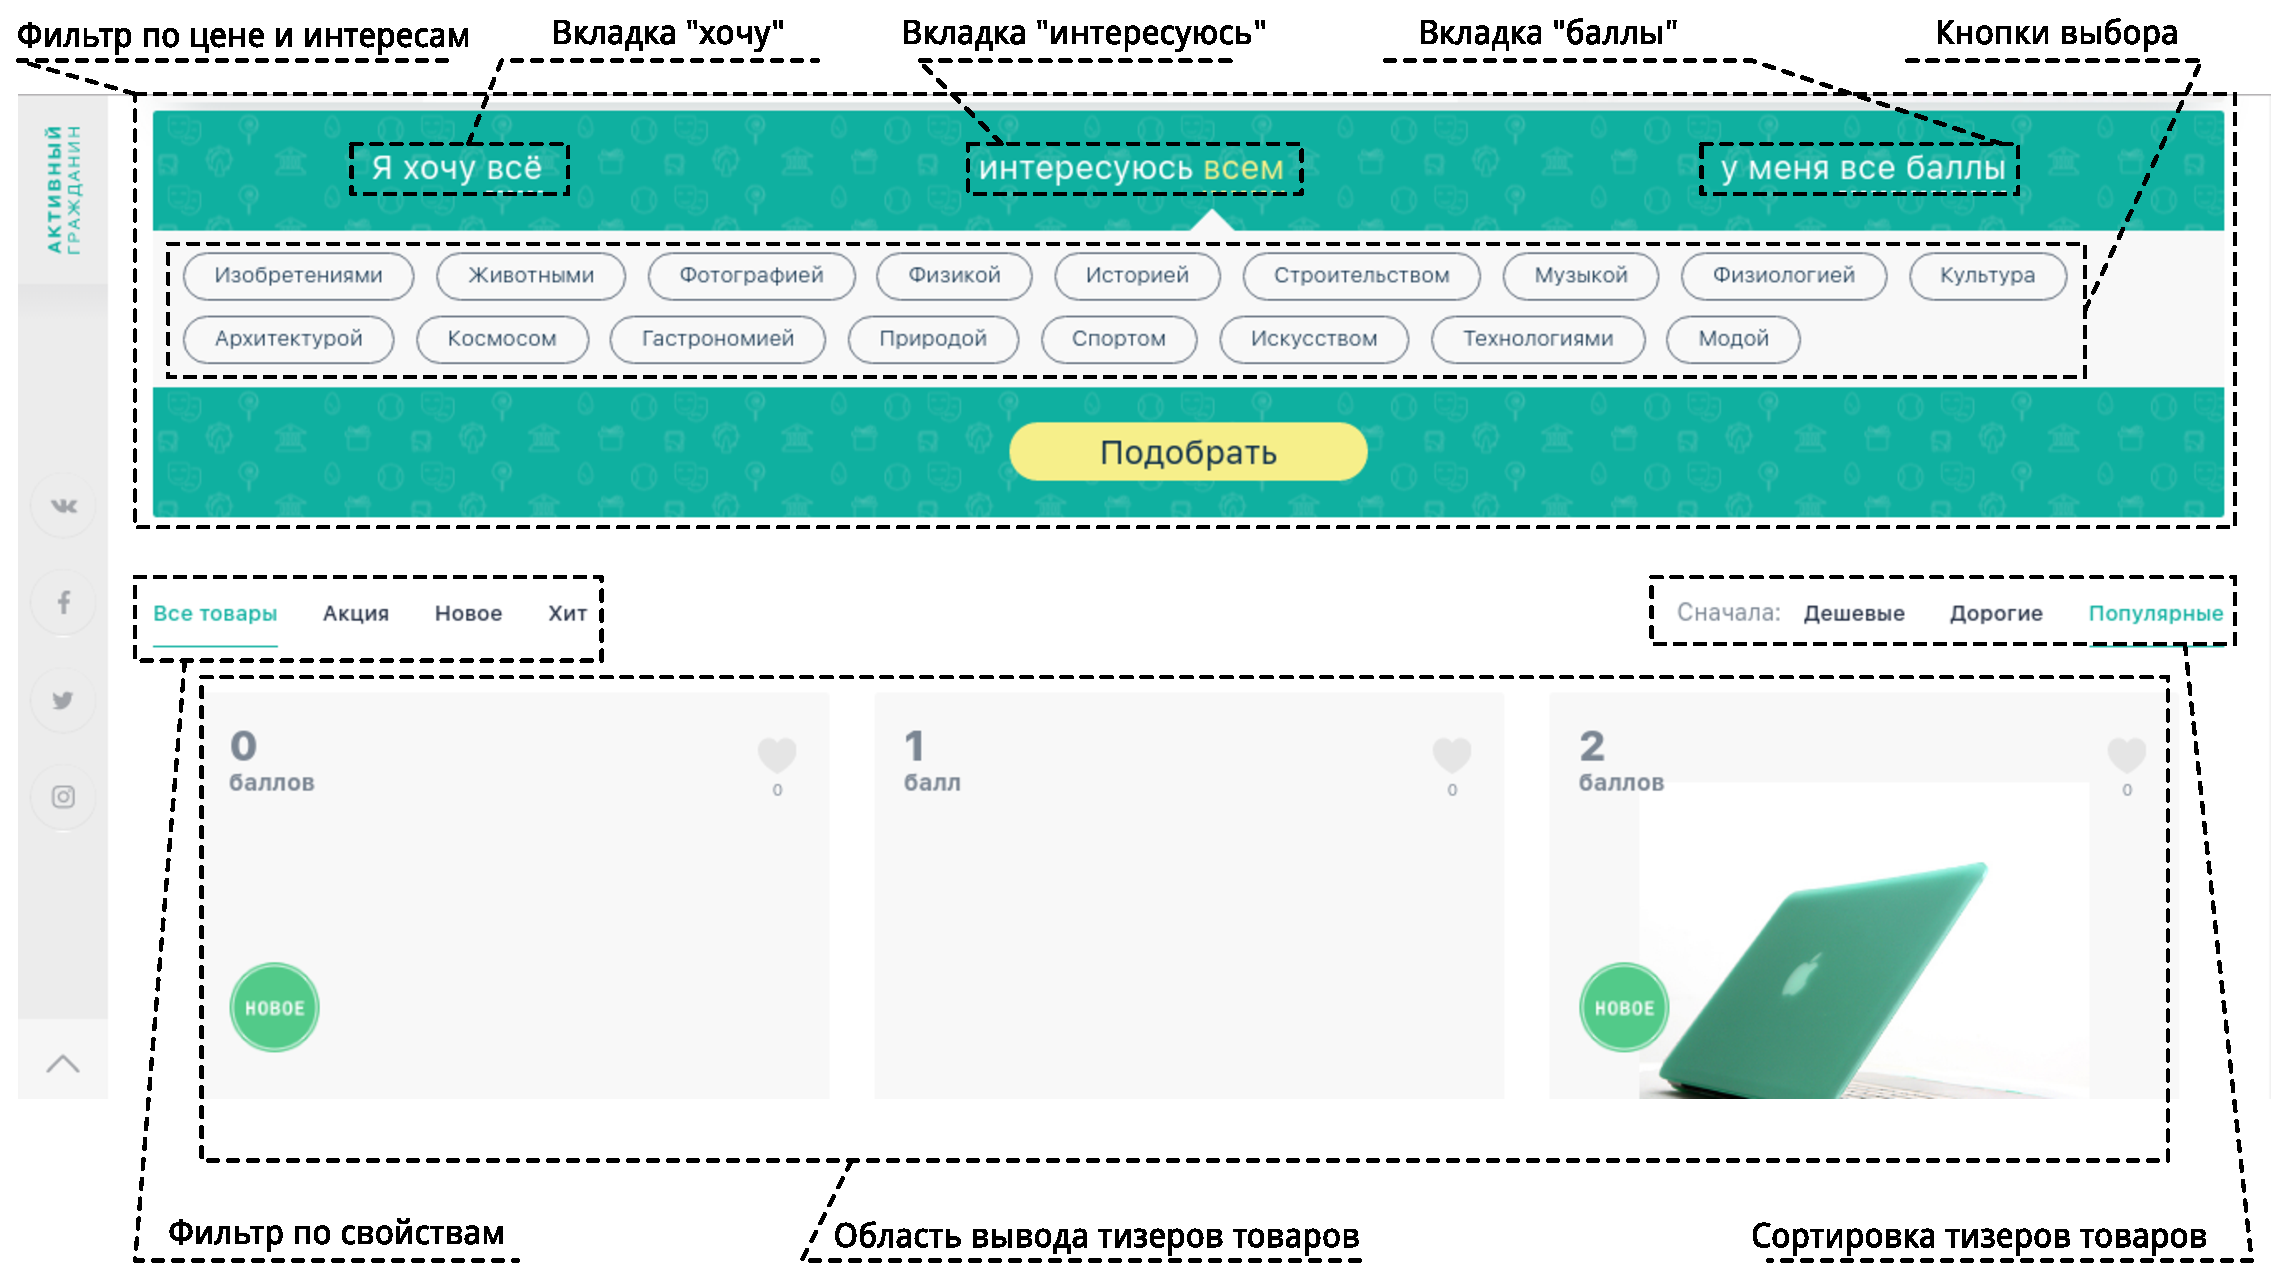
\includegraphics[width=170mm]{02_noauth_funcs/figures/02.eps}
            \caption{Фильтр по интересам и сортировка тизеров.}
            \label{fig:common_items_5}
        \end{figure}

        \begin{figure}
            \center
            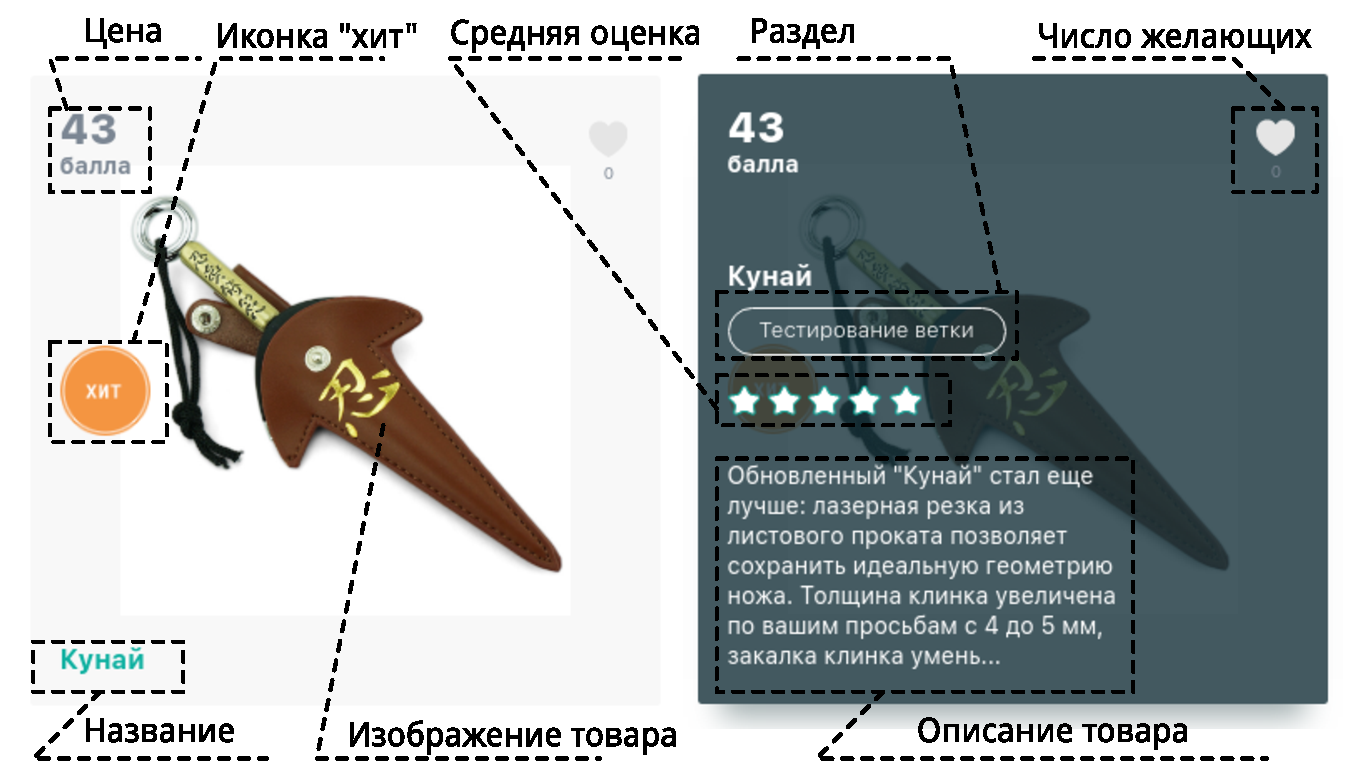
\includegraphics[width=170mm]{02_noauth_funcs/figures/05.eps}
            \caption{Тизер товара в пассивном состоянии и при наведении мыши.}
            \label{fig:common_items_4}
        \end{figure}


    \section{Главная страница}

        \begin{enumerate}
            \item
            Содержит следующие элементы
            \begin{itemize}
                \item Фиксированная панель слева (см. \ref{sec:baseitems_fixleft_panel})
                \item Главное меню (см. \ref{sec:baseitems_main_meu})
                \item Баннер-слайдер (см. \ref{sec:slider})
                \item Фильтр по цене и интересам (см. \ref{sec:baseitems_interest_filter})
                \item Ссылки фильтра по свойствам (см. \ref{sec:baseitems_props_filter})
                \item Ссылки сортировки списка тизеров товаров (см. \ref{sec:baseitems_goods_sort})
                \item Область вывода тизеров товаров (см. \ref{sec:baseitems_goods_area})
                \item Кнопка подгрузки.  (см. \ref{sec:baseitems_goods_more})
                \item Важные ссылки (см. \ref{sec:baseitems_important_links})
                \item Копирайт (см. \ref{sec:baseitems_footer_copiright})
            \end{itemize}
        \end{enumerate}
    
        \subsection{Банер-слайдер}
            см. рис. \ref{fig:common_items_1}
            \label{sec:slider}
            
            \begin{enumerate}
                \item В слайдере крутятся 2 вида слайдов: слайды-картинки и слайды-товары
                \item Тип слайда задаётся в \gloss{CMS}
            \end{enumerate}
            
            \subsubsection{Слайды-картинки}
                \paragraph{Изображение}
                    \begin{enumerate}
                        \item Картинка для отображения загружается в \gloss{CMS}
                        \item Картинка должна быть с соотношением сторон 87:50
                        \item Если при ином соотношении сторон картинка выводится таким образом, чтобы полностью заполнять слайд
                    \end{enumerate}
                
                \paragraph{Ссылка}

                    \begin{enumerate}
                        \item Ссылка может вести как на внутреннюю страницу магазина, так и на внешний ресурс
                        \item Ссылка открывается в новом окне
                    \end{enumerate}
               
            \subsubsection{Слайды-товары}
                \paragraph{Изображение}
                    \begin{enumerate}
                        \item В качестве ссылки на изображение берётся ссылка на главное фото товара
                    \end{enumerate}
                \paragraph{Ссылка}
                    \begin{enumerate}
                        \item Ссылка ведёт на карточку товара (см. \ref{sec:goods_cart})
                        \item Ссылка открывается в новом окне
                    \end{enumerate}
                \paragraph{Цена}
                \paragraph{Хит}
                \paragraph{Новое}
                \paragraph{Акция}
                \paragraph{Описание}
                \paragraph{Раздел}
                \paragraph{Ссылка с числом желающих}
            
        \begin{figure}
            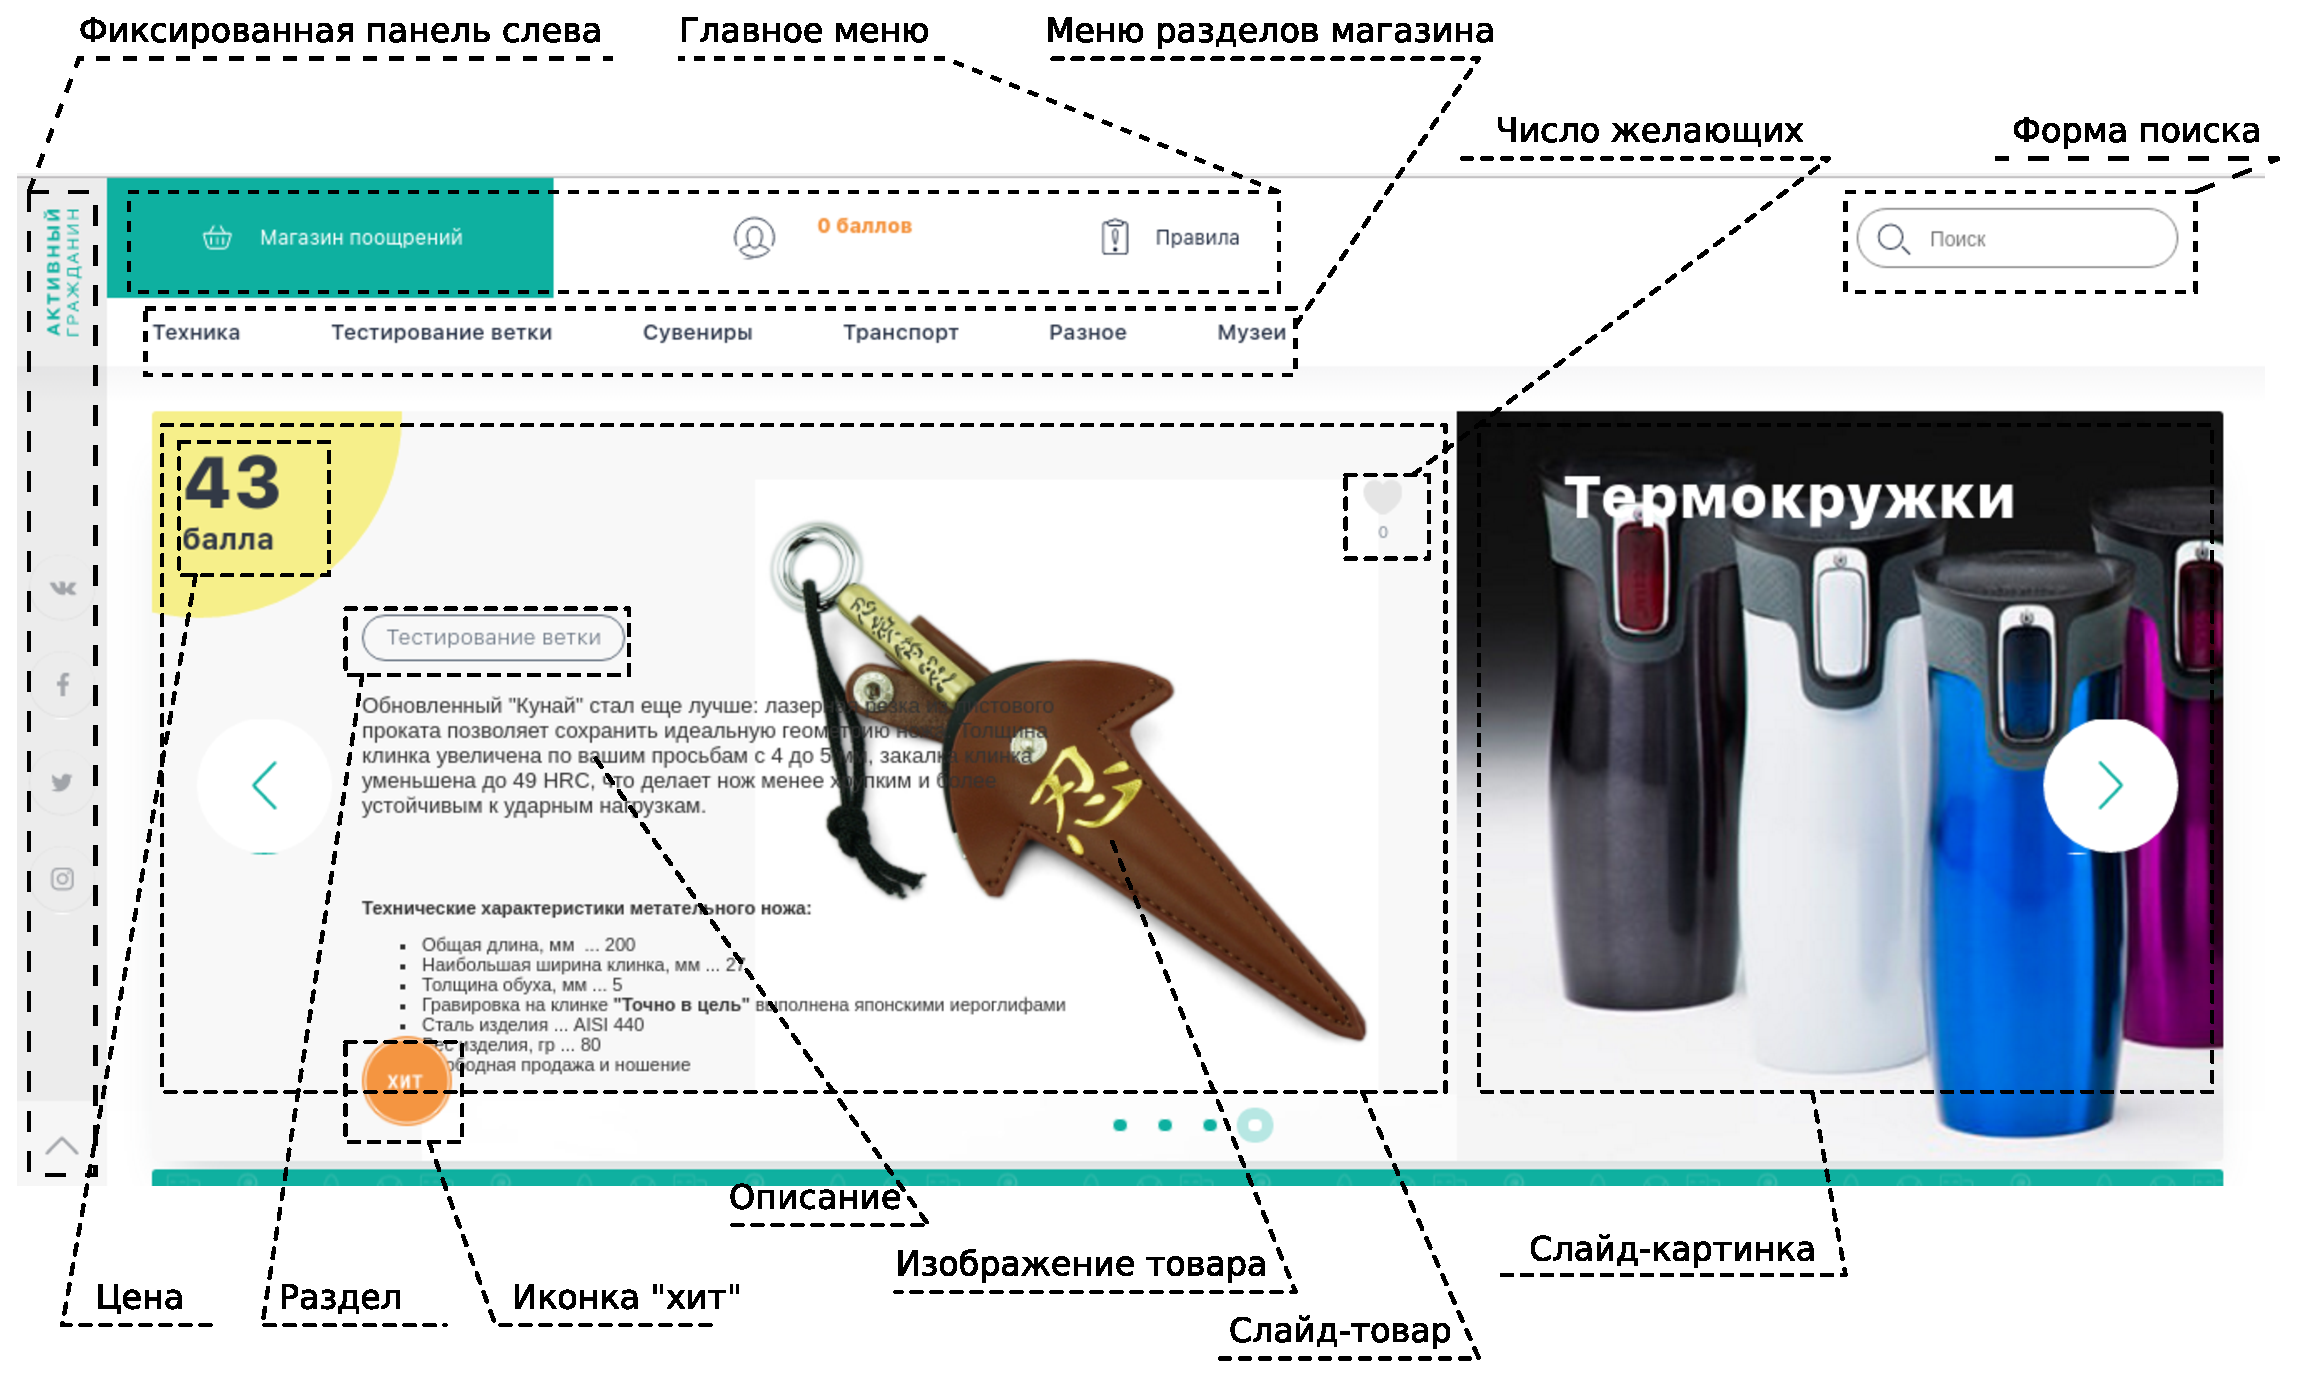
\includegraphics[width=170mm]{02_noauth_funcs/figures/01r.eps}
            \caption{Общие элементы страниц(верхняя часть страницы) и баннер-слайдер.}
            \label{fig:common_items_1}
        \end{figure}


    \section{Страницы разделов каталога}
        \label{sec:page_catalog_section}


    \section{Карточка товара}
        \label{sec:goods_cart}
        \subsection{Активное фото}
            \subsubsection{Иконка <<Новое>>}
            \subsubsection{Иконка <<Хит>>}
            \subsubsection{Иконка <<Акция>>}
            \subsubsection{Цена в баллах}
            \subsubsection{Число желающих.}

        \subsection{Панель навигации по фотографиям товара}
        \subsection{Средняя оценка товара}
        \subsection{Сообщение <<необходимо набрать N баллов>>}
        \subsection{Название товара}
        \subsection{Артикул}
        \subsection{Описание}
        \subsection{Сообщение <<срок действия вашего заказа>>}
        \subsection{Сообщение <<использовать до>>}
        \subsection{Отзывы.}

    \section{Правила}
        \subsection{Как это работает}
            \label{sec:rules_hiw}
        \subsection{Адреса}
        \subsection{FAQ}
            \label{sec:page_faq}

    \section{Страница поиска}
        \label{search_page}

